\section{評価結果}
今回倉庫棚を想定した棚での飛行実験は安定して想定通りの経路を飛行を行う事が出来た\footnote{\url{https://youtu.be/pw23Vq8DuHE}}.
具体的な飛行成績は以下の通りである.

\begin{table}[h]
    \caption{飛行結果}
    \label{table:fly_result}
    \centering
    \begin{tabular}{cccc}
        \hline
        試行回数 & 到達可否 & 周回時間[sec] & 平均位置補正時間[sec] \\
        \hline \hline
        1回目 & 可 & 214.58 & 12.22 \\
        2回目 & 可 & 199.19 & 10.08 \\
        3回目 & 可 & 225.43 & 12.35 \\
        4回目 & 可 & 242.86 & 14.20 \\
        5回目 & 可 & 289.67 & 19.44 \\
        6回目 & 可 & 294.40 & 19.97 \\
        7回目 & 可 & 285.03 & 18.93 \\
        8回目 & 可 & 265.28 & 16.76 \\

        9回目 & 可 & 214.58 & 12.22 \\
        10回目 & 可 & 214.58 & 12.22 \\
        \hline
    \end{tabular}
\end{table}

初回の位置合わせに時間がかかる事が多いものの,二つ目以降の位置合わせには時間差はあまり出なかった.
以下に90回分の位置補正にかかった時間の箱日げ図を示す.\ref{box_plot}

\begin{figure}[htbp]
    \begin{center}
      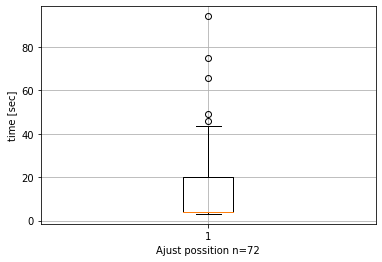
\includegraphics[clip,width=15.0cm]{img/timedata.png}
      \caption{位置補正に要した時間}
      \label{box_plot}
    \end{center}
  \end{figure}